\documentclass[12pt,a4paper,oneside]{book}
\usepackage[left=2cm,right=2cm,top=3cm, bottom=3cm]{geometry}
\usepackage[utf8]{inputenc}
\usepackage{graphicx}
\usepackage{fancyhdr}
\usepackage[spanish]{babel}
\usepackage{amsmath}
\usepackage{amssymb}
\author{Axel Aveiga Defaz}
\title{Teoremas de Geometría}

% \begin{figure}
% \lhead{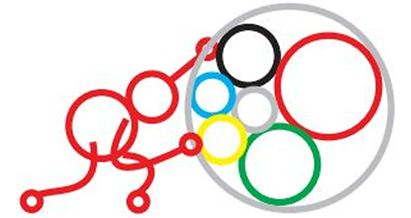
\includegraphics[scale=0.25]{Imagenes/image001.png}}
% \end{figure}
% \rhead{\LaTeX\ por Axel Aveiga
% \\Liceo Cristiano de Guayaquil}

\begin{document}
\maketitle

\setlength{\parindent}{0 pt}
\renewcommand{\headrulewidth}{0.5pt}
\cfoot{}

\tableofcontents
\let\cleardoublepage\clearpage

\chapter{Teoremas de Geometría.}
\section{Teorema de suma de los ángulos de un triángulo.} 
La suma de los ángulos internos de un triángulo es $180^\circ$.
\section{Desigualdad del triángulo.}
Sean $a, b$ y $c$ las longitudes de los lados de un triángulo, si y sólo si, 
$$a+b>c,$$ 
$$a+c>b,$$ 
$$b+c>a$$
\section{Primer teorema de Thales.}
En un triángulo $ABC$, sean $D$ y $E$ puntos en $AB$
y $AC$ respectivamente, $DE$ es paralela a $BC$ si y sólo si $$\dfrac{AB}{AD}=\dfrac{AC}{AE}$$
\section{Segundo teorema de Thales.}
Se considera tres rectas y dos rectas transversales a éstas como se muestra en la figura. $AD, BE$ y $CF$ son paralelas si y sólo si $\dfrac{AB}{BC}=\dfrac{DE}{EF}$.
\begin{center}
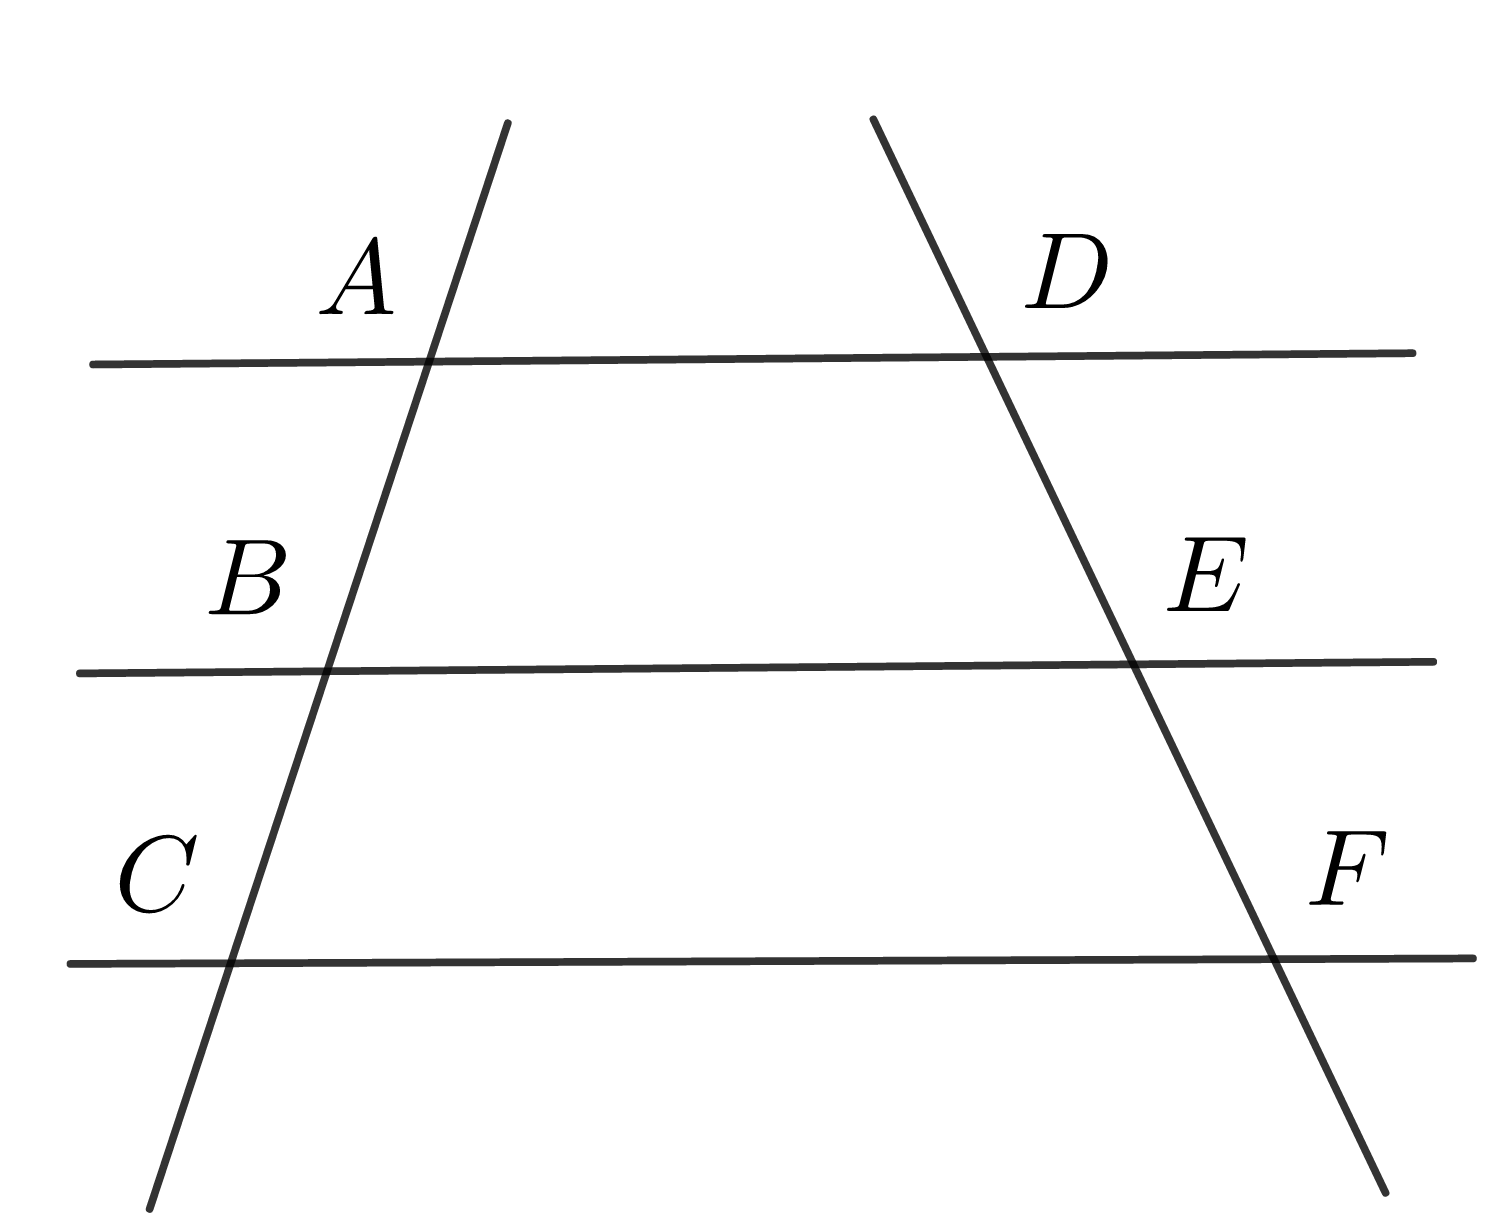
\includegraphics[scale=0.45]{Imagenes/thales.png}
\end{center}
\newpage
\section{Teorema de semejanza $\angle -\angle -\angle$.}
Si dos triángulos tienen todos sus ángulos correspondientes iguales entonces sus lados correspondiente son proporcionales y los triángulos son semejantes.
\section{Teorema de semejanza $L-\angle - L.$}
Si dos triángulos tienen dos lados correspondientes proporcionales y el ángulo comprendido entre éstos es igual, entonces son semejantes.
\section{Teorema de semejanza $L-L-L$.}
Si dos triángulos tienen sus lados correspondientes proporcionales entonces los triángulos son semejantes.
\section{Teorema de Pitágoras.}
Un triángulo es rectángulo si y sólo si el cuadrado de la hipotenusa es igual a la suma de los cuadrados de los catetos.
\section{Teorema del Baricentro.}
Las medianas de un triángulo son concurrentes en un punto conocido como el Baricentro.
\section{Teorema del Incentro.}
Las bisectrices internas de un triángulo son concurrentes en un punto conocido como el Incentro.
\section{Teorema del Circuncentro.}
Las mediatrices de los lados de un triángulo son concurrentes en un punto conocido como el Circuncentro.
\section{Teorema del Ortocentro.}
Las alturas de un triángulo son concurrentes en un punto conocido como el Ortocentro.
\section{Teorema de la medida del ángulo inscrito.}
La medida de un ángulo inscrito en una circunferencia es igual a la mitad del arco comprendido entre sus lados, es decir, es la mitad del ángulo central que abre del mismo arco.
\section{Teorema de la medida del ángulo semi-inscrito.}
Todo ángulo semi-inscrito es igual a la mitad del ángulo central que abarca el mismo arco.
\section{Teorema de cuadrilátero cíclico.}
\begin{enumerate}
\item Un cuadrilátero convexo es cíclico si sólo si sus ángulos opuestos son suplementarios.
\item Un cuadrilátero convexo es cíclico si sólo si el ángulo entre un lado y una diagonal es igual al ángulo entre el lado opuesto y la otra diagonal.
\end{enumerate}
\section{Ley del paralelogramo.}
La suma de los cuadrados de las diagonales de un paralelogramo es igual a la suma de los cuadrados de sus lados, es decir, si $d_1$ y $d_2$ son las diagonales y $a, b$ los lados, entonces tenemos que 
$$d_1^2 + d_2^2=2a^2+2b^2$$
\section{Teorema de la recta de Euler.}
En un triángulo $ABC$ el ortocentro, el centroide y el circuncentro son colineales. La recta donde se encuentran estos puntos se conoce como la recta de Euler.
\section{Teorema de la circunferencia de nueves puntos.}
Los pies de las tres alturas de un triángulo, los puntos medios de los tres lados y los puntos medios de los segmentos que van de los vértices al ortocentro, están en una circunferencia de radio $\dfrac{1}{2}R$, donde $R$ es el radio del circuncentro del triángulo $ABC$.
\section{Teorema del centro de la circunferencia de nueve puntos.}
El centro de la circunferencia de nueve puntos se encuentra en la recta de Euler y es el punto medio del segmento $HO$, donde $H$ y $O$ es el ortocentro y circuncentro, respectivamente.
\section{Teorema de Ceva.}
En un triángulo $ABC$ los puntos $D$, $E$, $F$ sobre los lados $BC$, $AC$, y $AB$, respectivamente. Las rectas $AD$, $BE$ y $CF$ concurren en un punto si y sólo si
$$\dfrac{BD}{DC}\cdot\dfrac{CE}{EA}\cdot\dfrac{AF}{FB}=1$$
\section{Teorema de Menelao.}
En un triángulo $ABC$, una recta intersecta las rectas $BC$, $CA$ y $AB$ en los puntos $D$, $E$ y $F$ si y sólo si
$$\dfrac{BD}{DC}\cdot\dfrac{CE}{EA}\cdot\dfrac{AF}{FB}=-1$$
\section{Teorema de la bisectriz.}
Sea un triángulo $ABC$, la bisectriz $AL$, donde $L$ es la intersección de la bisectriz con $BC$, del ángulo en $A$ divide al lado opuesto $BC$ de tal forma que
$$\dfrac{BL}{LC}=\dfrac{AB}{CA}$$
\section{Teorema de Pappus.}
Si $A$, $C$, $E$ son tres puntos en una recta, $B$, $D$, $F$ tres puntos en otra recta $AB$, $CD$, $EF$ intersectan a las rectas $DE$, $FA$ y $BC$ respectivamente, entonces los tres puntos de intersección $L$, $M$ y $N$ son colineales.
\section{Teorema de Desargues.}
Si dos triángulos están perspectivas desde un punto y si sus pares de lados correspondientes si intersectan, entonces los tres puntos de intersección.
\section{Teorema recíproco de Desargues.}
Si dos triángulos están están en perspectivas desde una recta, entonces las rectas que unen dos pares de vértices correspondientes son concurrentes; por lo que los triángulos están en perspectiva desde el punto de intersección de estas rectas.
\section{Teorema de Desargues con paralelas.}
Si $PQR$ y $P'Q'R'$ son dos triángulos  en perspectiva desde un punto y éstos tienen dos pares de lados correspondientes paralelos entonces los otros dos lados correspondientes paralelos entonces los otros dos lados correspondientes son paralelos. Recíprocamente, si los triángulos $PQR$ y $P'Q'R'$ tienen lados correspondientes paralelos y dos rectas que unen puntos correspondientes se intersectan en un punto $O$ entonces los triángulos están en perspectiva desde $O$.
\section{Teorema del centro de gravedad.}
El centroide $G$ es el único punto dentro del triángulo $ABC$ que tiene la propiedad de que los triángulos $BCG$, $CAG$ y $ABG$ tienen la misma área.
\section{Teorema del triángulo órtico.}
El ortocentro de un triángulo acutángulo es el incentro del triángulo órtico.
\section{Teorema del Excentro.}
Las bisectrices externas de cualesquiera dos ángulos de un triángulo son concurrentes con la bisectriz interna del tercer ángulo.
\section{Identidades pitágoricas.}
Sea $\alpha$ un ángulo cualquiera,$$\cos^ 2 \alpha + \sin ^2 \alpha =1$$
\section{Suma y diferencias de ángulos en el seno y coseno.}
Sea $\alpha$ y $\beta$ dos ángulos cualesquiera, se cumple que:$$\cos ( \alpha \pm \beta) = \cos \alpha \cos \alpha \mp \sin \alpha \sin \beta$$
$$\sin (\alpha \pm \beta) = \cos \alpha \sin \beta \pm \cos \beta \sin \alpha$$
\section{Ley de cosenos.}
Sea un triángulo con $a$, $b$ y $c$ las longitudes de los lados y $\beta$ el ángulo opuesto al lado $b$.
$$b^2 = a^2 + c^2 -2ac \cos \beta$$
\section{Ley de senos.}
Sea $ABC$ un triángulo inscrito en una circunferencia de radio $R$. Si $a$, $b$ y $c$ son los lados del triángulo opuestos a los vértices $A$, $B$ y $C$ respectivamente, entonces$$ \dfrac{a}{\sin A} = \dfrac{b}{\sin B}= \dfrac{c}{\sin C}= 2R$$
\section{Teorema de Stewart.}
Sean $ABC$ un triángulo y $AX$ una ceviana de longitud $p$, que divide al segmento $BC$ en dos segmentos $BX=m$ y $XC=n$; $$a(p^2 +mn) = b^2m + c^2n$$
\begin{center}
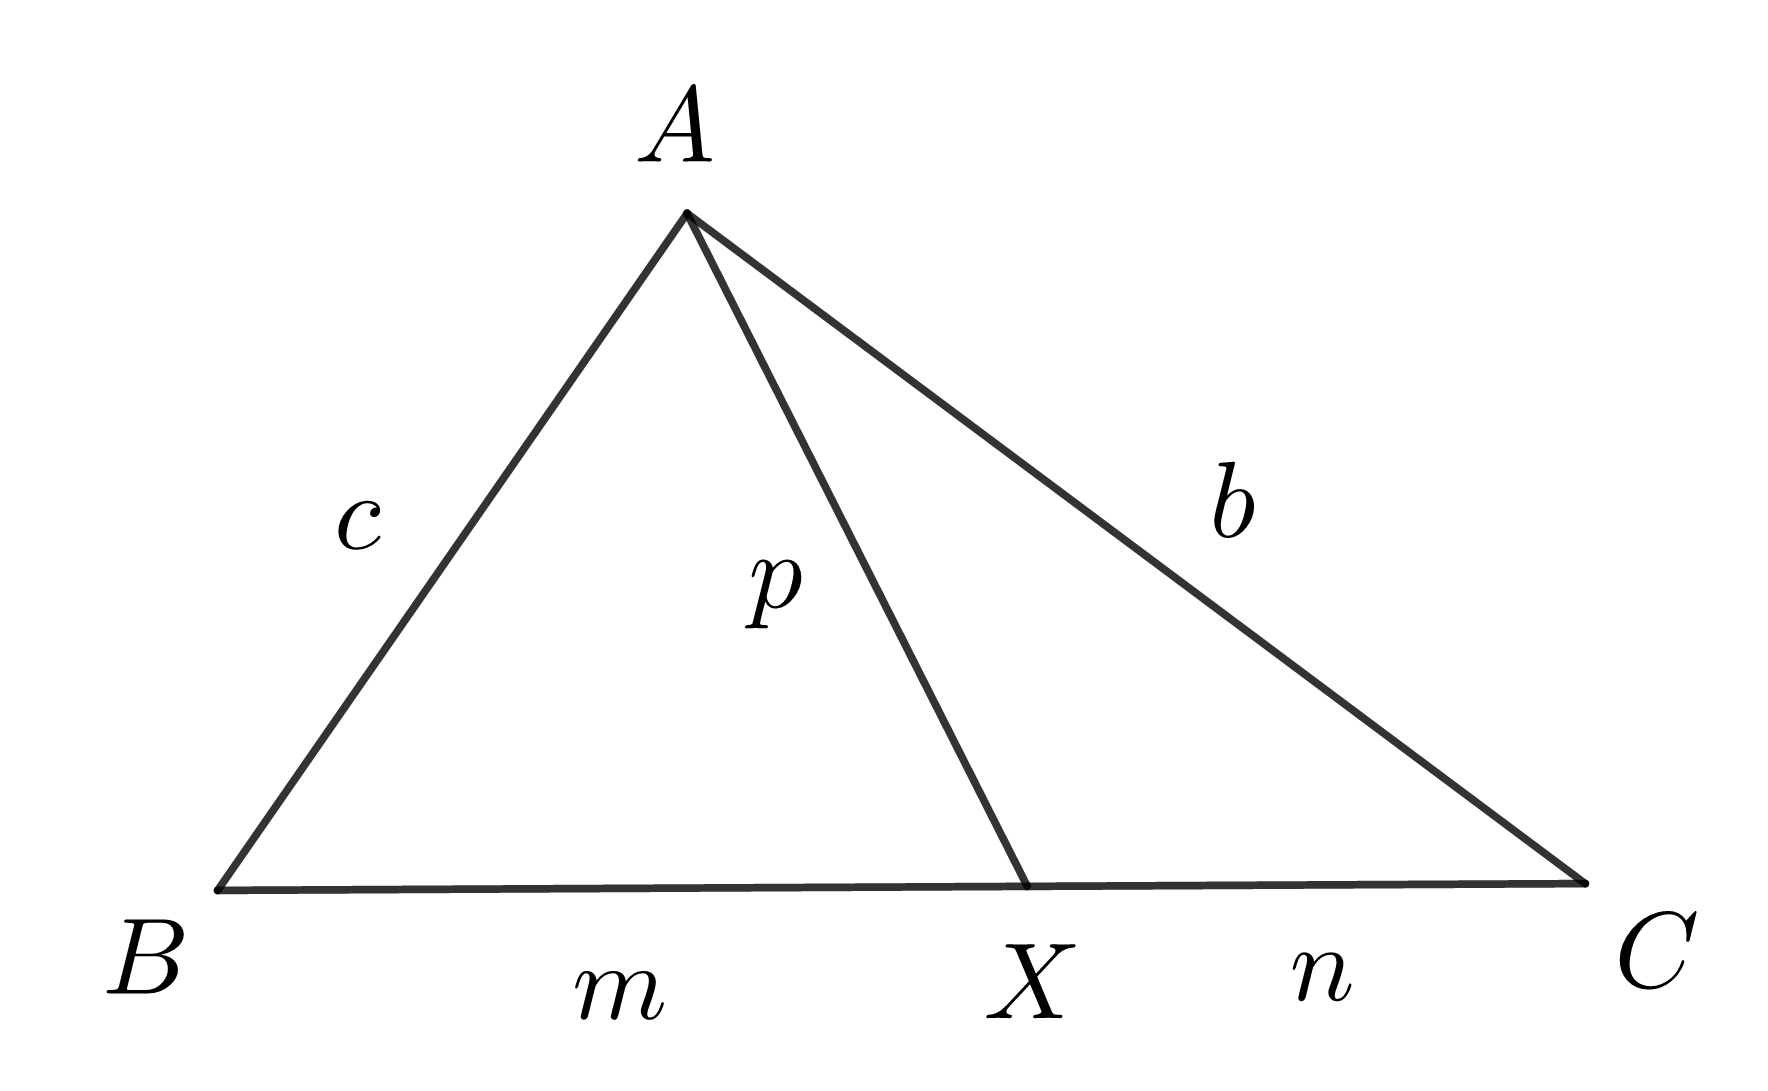
\includegraphics[scale=0.6]{Imagenes/stewart.png} 
\end{center}
\section{Fórmulas del área de un triángulo.}
Sea $ABC$ un triángulo con lados de longitud $a$, $b$, y $c$. Si $s$, $r$ y $R$ son el semiperímetro, el inradio y el circunradio del triángulo, respectivamente: Entonces su área las podemos calcular como:
\begin{eqnarray*}
(ABC)&=& \dfrac{ac \sin \angle CBA}{2}
\\(ABC)&=& \dfrac{abc}{4R}
\\(ABC)&=& sr
\\(ABC)&=& \sqrt{s(s-a)(s-b)(s-c)}
\end{eqnarray*}
\section{Desigualdad geométrica.}
Si $a$, $b$, $c$ son los lados de un triángulo de área $(ABC)$ entonces $$4\sqrt{3}(ABC) \leq a^2 + b^2 + c^2$$
\\con igualdad si y sólo si $a$, $b$, $c$ es equilátero.
\section{Desigualdad de Nesbitt.}
Sea $a$, $b$ y $c$ números positivos, se cumple que:
$$\dfrac{a}{b+c} + \dfrac{b}{c+a}+ \dfrac{c}{a+b} \geq \dfrac{3}{2}$$
\section{Transformación de Ravi.}
Sea $a$, $b$ y $c$ lados del triángulo, entonces $a=x+y, b=y+z, c=z+x$ con $x$, $y$, $z$ pertenecientes a los reales positivos.
\section{Desigualdad geométrica.}
Sean $A$, $B$ y $C$ ángulos de un triángulo, $$\cos A +\cos B +\cos C \leq \dfrac{3}{2}$$ 
\section{Teorema de Potencia de Punto.}
Si las cuerdas $AB$ y $CD$ son cuerdas; $A, B, C, D$ están sobre una misma circunferencia, si y sólo si intersectan en un punto $P$ y cumple que $$PA \cdot PB = PC \cdot PD$$
\section{Teorema del Centro Radical.}
Los ejes radicales de tres circunferencias se intersectan en un punto $P$.
\section{Teorema de Fórmula de Euler.}
Una condición necesaria y suficiente para la existencia de un triángulo con circuncírculo $( O, R)$ e incírculo $(I, r)$ es la igualdad $$OI ^2= R^2 - 2Rr$$
\section{Teorema de Homotecia.}
Dos circunferencias de radio  y centros distintos, son figuras homotéticas.
\section{Teorema de la Circunferencia de Apolonio.}
Si $A$, $B$ son dos puntos fijos y $\dfrac{p}{q}$ es una razóin fija, el lugar geométrico de los puntos $P$ que sastifacen $\dfrac{AP}{PB}=\dfrac{p}{q}$ es una circunferencia.
\section{Teorema de Inversión.}
Sea $C=(O, r)$ una circunferencia de inversión. 
\begin{enumerate}
\item Una recta que pasa por $O$, se invierte en ella misma.
\item El inverso de una recta que no pasa por $O$, es una circunferencia que pasa por $O$
\item El inverso de una circunferencia que pasa por $O$, es una recta que no pasa por $O$.
\item El inverso de una circunferencia que no pasa por el centro de inversión $O$ es una circunferencia que no pasa por $O$.
\end{enumerate}
\section{Teorema de circunferencias  ortogonales.}
Circunferencias ortogonales se invierten en circunferencias ortogonales.
\section{Fórmula de Inversión.}
Sean $C(O. r)$ una circunferencia de inversión, $P$, $Q$ dos puntos del plano y $P'$, $Q'$ sus puntos inversos, entonces.$$Q'P'= \dfrac{r^2PQ}{OP \cdot OQ}$$
\section{Teorema de Varignon.}
Los puntos medios de los lados de un cuadrilátero son los vértices de un paralelogramo. El perímetro del paralelogramo es igual a la suma de las longitudes de la diagonales y su área es igual a la mitad del área del cuadrilátero. 
\section{Teorema de Ptolomeo.}
El cuadrilátero $ABCD$ es cíclico si y sólo si $$AC \cdot BD = AB \cdot CD + BC \cdot AD$$.
\section{Teorema extendido de Ptolomeo.}
Para cuatros puntos $A$, $B$, $C$ y $D$ siempre es válida la desigualdad:$$AB \cdot DC + BC\cdot DA \geq CA \cdot DB$$ 
y la igualdad se da solamente en el caso que $A$, $B$, $C$ y $D$ sean concíclicos.
\section{Teorema de Simson.}
Las proyecciones de un punto sobre los lados de un triángulo son colineales si y sólo si el punto se encuentra sobre el circuncírculo del triángulo.
\section{Teorema del perímetro de un cuadrilátero.}
Entre los cuadriláteros de perímetro dado el cuadrado es el de mayor área.
\section{Teorema de Pitot.}
El cuadrilátero $ABCD$ es circunscrito si y sólo si $$AB + CD = BC +DA$$
\section{Teorema de Brahmagupta.}
En un cuadrilátero cíclicos con diagonales perpendiculares, al que llamamos ortodiagonal, la recta que pasa por el punto de intersección de las diagonales y es perpendicular a un lado biseca al lado opuesto.
\section{Teorema de Brahmagupta (Área).}
El área $A$ de un cuadrilátero cíclico de lados $a$, $b$, $c$, $d$ y semiperímetro $s$ está dada por $$A^2=(s-a)(s-b)(s-c)(s-d)$$
\section{Teorema del Punto de Miquel.}
Sea $ABC$ un triángulo, con puntos arbitrarios $A'$, $B'$ y $C'$ en lados $BC$, $AC$ y $AB$ , respectivamente. Dibuje tres circunferencias circunscritas a los triángulos $AB'C'$, $A'BC'$ y $A'B'C$. Estos círculos se intersectan en un punto $M$.
\section{Teorema de Gergonne.}
Si el incircírculo de un triángulo $ABC$ es tangente a los lados $BC$, $CA$ y $AB$ en los puntos $X$, $Y$ y $Z$,respectivamente, entonces las cevianas  $AX$, $BY$ y $CZ$ son concurrentes en un punto $G.$
\section{Teorema de Nagel.}
Sea un triángulo $ABC$. Los puntos $L$, $M$ y $N$ están sobre los lados $BC$, $CA$ y $AB$ tales que $AB + BL = LC + CA, BC + CM= MA + AB$ y $CA + AN= NB + BC$, entonces $AL, BM$ y $CN$ son concurrentes.
\section{Teorema de Blanchet.}
Sea un triángulo $ABC$ y sea $H$ la base de la altura $C$. $AX$, $BY$ y $CH$ se intersectan un punto $P$, con $X$ y $Y$ puntos sobre los lados $BC$ y $CA$, respectivamente, entonces $$\angle CHY = \angle CHX$$
\section{Teorema de la Mariposa.}
Sea $M$ el punto medio de la cuerda $AB$. Las cuerdas $CD$ y $EF$ pasan por $M$. $CF$ y $ED$ intersectan a $AB$ en $U$ y $V$ respectivamente, entonces $M$ también el punto medio de $UV$.
\section{Teorema de Viviani.}
Sea $ABC$ un triángulo equilátero con altura $h$. Sea $P$ un punto arbitrario dentro del triángulo $ABC$. Si $X, Y$ y $Z$ son las perpendiculares que van desde $P$ hacia $BC$, $CA$ y $AB$, respectivamente, entonces $$PX + PY +PZ = h$$
\section{Teorema de Vecten.}
Sea un triángulo $ABC$. Se construye cuadrados externamente al triángulo sobre los lados $BC$, $CA$, $AB$ con centros $X$, $Y$, $Z$, respectivamente. Entonces $AX$, $BY$ y $CA$ son concurrentes.
\section{Teorema de Van Aubel.}
Sea un cuadrilátero $ABCD$. Se trazan cuadrado externos al cuadrilátero sobre los lados $AB$, $BC$, $CD$, $DA$ con centros $W$, $X$, $Y$, $Z$ respectivamente. Entonces $WY= XZ$ y $WY$ es perpendicular $XZ$
\section{Teorema de la cuaterna armónica.}
Sea $A, B$ y $C$ puntos en una misma recta $l$, en ese orden.  Sea $X$ un punto que no este sobre $l$. Sean $Y$ y $Z$ las intersecciones de los segmentos $AX$ y $BX$ y una recta que pase por $C$, respectivamente. Sea $P$ la intersección de $AZ$ con $YB$. Si $XP$ intersecta a $l$ en $D$ entonces se cumple que $$AD \cdot BC= AC \cdot DB$$
\section{Teorema del punto cicloceviano conjugado.}
Sea $ABC$ un triángulo con puntos puntos $X$, $Y$, $Z$ sobre ${BC}$, ${CA}$ y ${AB}$, respectivamente, tales que $AX$, $BY$ y $CZ$ sean colineales. Los puntos $X'$, $Y'$, $Z'$ son las intersecciones del circuncírculo del triángulo $XYZ$ con $AX$, $BY$ y $CZ$ respectivamente. Entonces $AX'$, $BY'$ y $CZ'$ son colineales.
\section{Teorema de Monge.}
Sean 3 circunferencias con centro $A$, $B$, $C$ no colineales, que cumple que sus centros y radios son diferentes. Los puntos $X$, $Y$, $Z$ son la intersección de la tangentes externas de los círculos con centro $A$ y $B$, $B$ y $C$, $C$ y $A$ respectivamente. Entonces $X$. $Y$, $Z$ son colineales. 
\section{Teorema del Hexágono Místico de Pascal.}
Sea $ABCDEF$ un hexágono cíclico. Los puntos $X$, $Y$, $Z$ son las intersecciones de $AF$ con $CD$, $AB$ con $DE$, $BC$ con $EF$; respectivamente. Entonces $X$, $Y$, $Z$ son colineales.
\section{Teorema de los círculos de Jhonson.}
Sean tres circunferencias de radio iguales que pasan por un punto $P$. Sin perdida de generalidad, sean $X$, $Y$, $Z$ las intersecciones de los pares de circunferencias diferentes $P$. El circuncírculo del triangulo $XYZ$ es congruente con las 3 circunferencias.
\section{Teorema de Bevan.}
Sea un triángulo $ABC$ con excentros $E_A, E_B$ y $E_C$. Las rectas $L_A, L_B$ y $L_C$ que pasan por los excentros y son perpendiculares al correspondientes lado del triángulo, son concurrentes.
\section{Teorema de Brocard.}
Sea $ABCD$ un triángulo cíclico. Sea $O$ el centro de la circunferencia del cuadrilátero $ABCD$. Los puntos $P$, $Q$ y $R$ son las intersecciones de $AB$ con $CD$, $BC$ con $AD$ y $AC$ con $BD$. Entonces el ortocentro del triángulo $PQR$ es $O$. 
\section{Teorema de Adam.}
El incircírculo con incentro $I$ de un triángulo $ABC$ es tangente a los lados $BC$, $CA$ y $AB$ en los puntos $X$, $Y$, $Z$ respectivamente. Las cevianas  $AX$, $BY$ y $CZ$ son concurrentes en un punto $G.$ Las rectas paralelas a $XY$, $YZ$, $ZX$ que pasan por $G$, intersectan a $AB$, $BC$ y $CA$ en $P$ y $Q$, $R$ y $S$, $T$ y $U$; respectivamente. Entonces el hexagono $PQRSTUV$ es concíclico con centro $I$.
\section{Teorema de la Hire.}
Si $Q$ pertenece a la polar de $P$, entonces $P$ pertenece a la polar de $Q$.

\chapter{Demostraciones}
\section{Teorema de suma de los ángulos de un triángulo.} 
La suma de los ángulos internos de un triángulo es $180^\circ$.
\\
\begin{center}
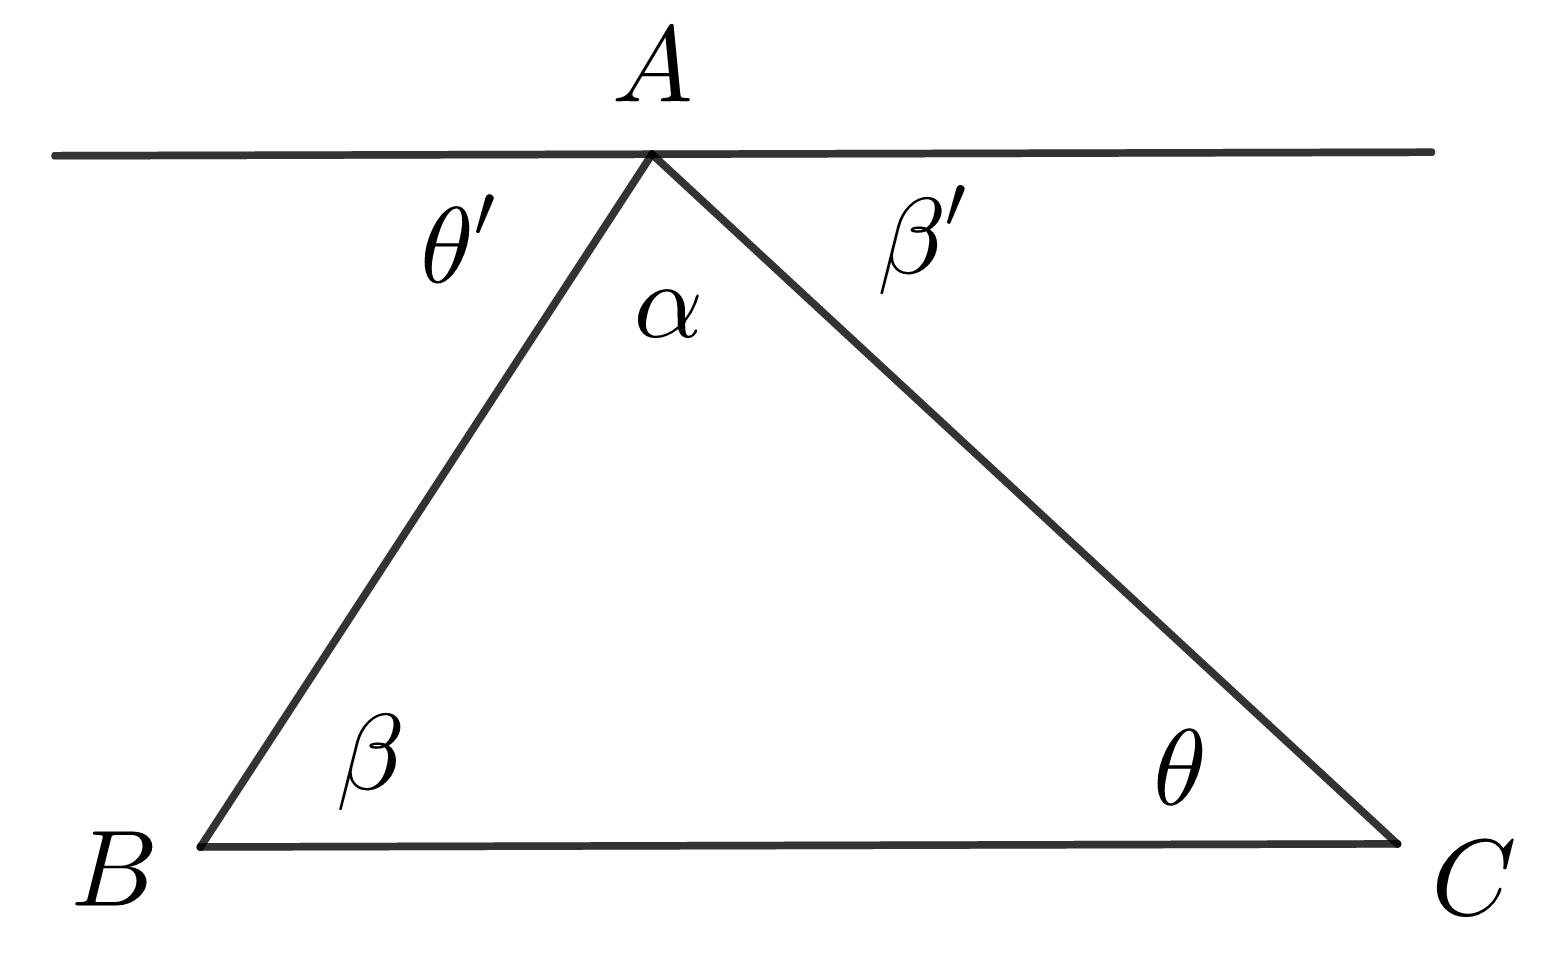
\includegraphics[scale=0.7]{Imagenes/demo1.png}
\end{center}
\begin{tabular}{p{15.9cm} p{1cm}}
Sea un triángulo $ABC$, por el vértice $A$ trazamos una recta paralela al lado $BC$. 
\\Definimos el $\angle A=\alpha, \angle B=\beta$ y $\angle C= \theta$ y definimos respectivamente los  ángulos alternos internos que están en la paralela a $BC$ como $\beta '$ y $\theta '$. & \medskip (1)
\\Por definición y ser ángulo alternos internos, $\beta= \beta '$ y $\theta=\theta '$ &(2)
\\Por (1), los ángulos $\alpha,\beta'$ y $\theta'$ forman un ángulo llano. & (3)
\\Por (2) y (3), $\alpha + \beta+ \theta = \alpha + \beta '+ \theta ' = 180^ \circ$ &(4)
\\Por (4), los  ángulos internos de un triángulo sumas $180^\circ$
\end{tabular}
\section{Desigualdad del triángulo.}
Sean $a, b$ y $c$ las longitudes de los lados de un triángulo, si y sólo si, 
$$a+b>c,$$ 
$$a+c>b,$$ 
$$b+c>a$$
\begin{center}
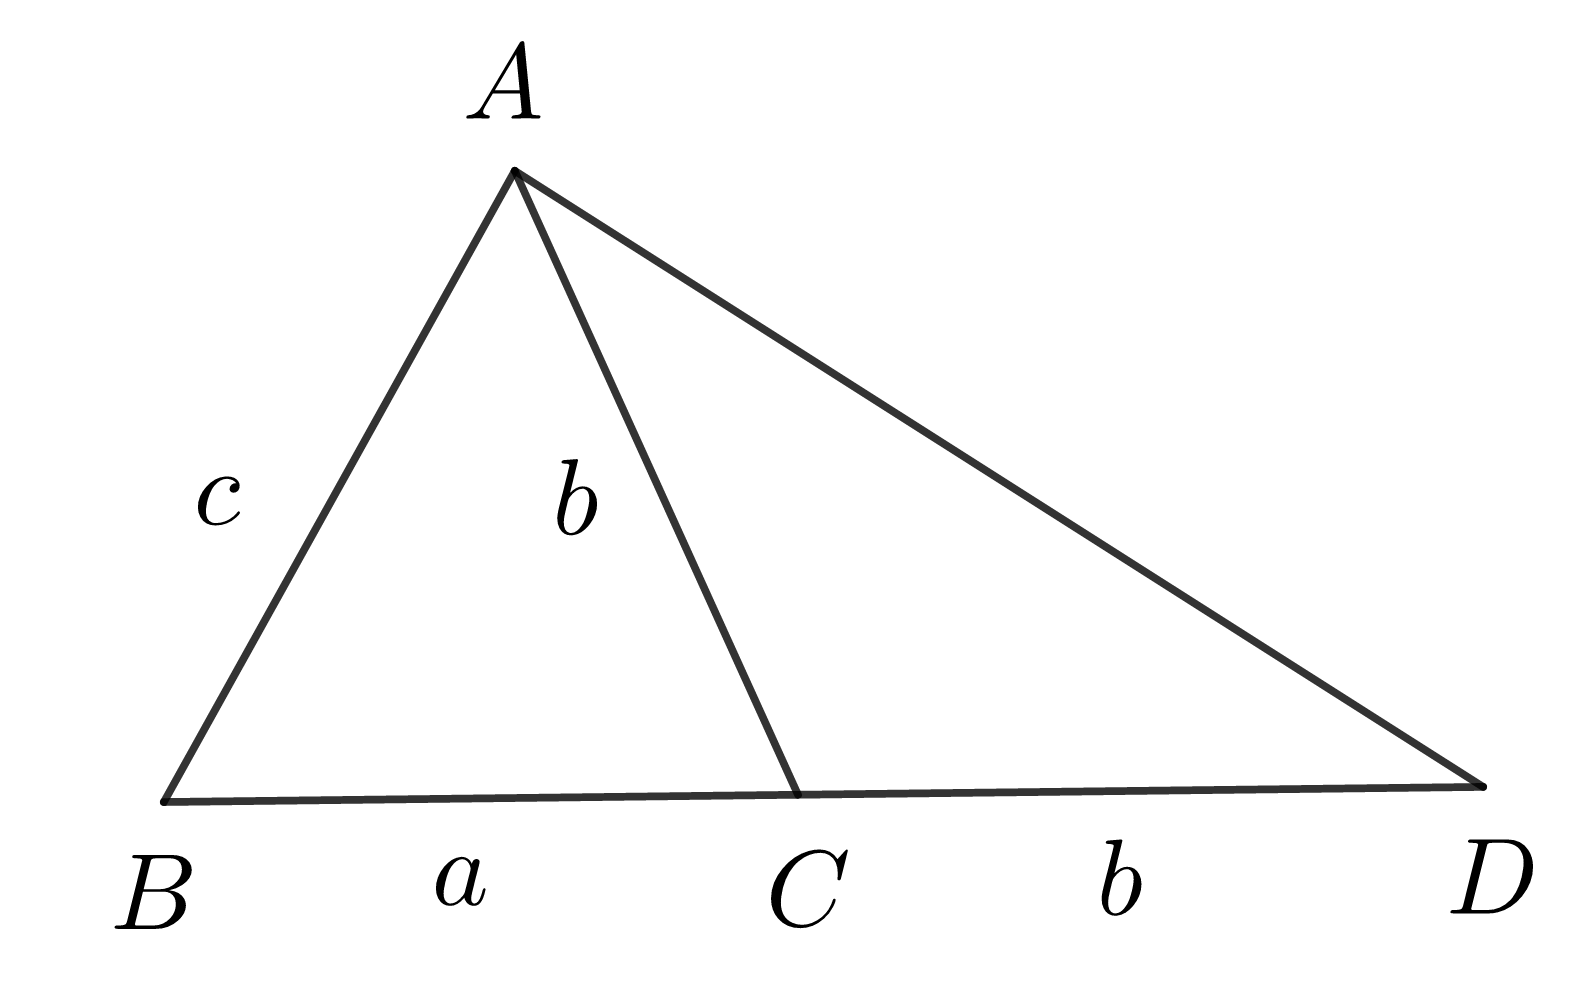
\includegraphics[scale=0.7]{Imagenes/demo2.png} 
\end{center}
\begin{tabular}{p{15.9cm} p{1cm}}\\
Sea $D$ un punto sobre la prolongación del lado $BC$ del triángulo $ABC$, tal que $AC=CD$ & (1)
\\Por (1), $BD=BC+CD=a+b$ & (2)
\\Por (2), el triángulo $ADC$ es isósceles & (3) 
\\Por (3) y $\angle BAD =\angle BAC +\angle CAD$, $\angle BAD > \angle CAD = \angle CDA$ &(4)
\\Se  demostrará lo siguiente, si un triángulo $ABC$ se cumple que $\angle A > \angle B$ entonces $a > b$. &(*)
\\Sea $D$ un punto sobre $AC$ tal que $CD=CB$.
\\Como $\angle A > \angle B$, el punto $D$ no está sobre $\overline{AC}$ & (5)
\\Por (5) y definición de $D$, $CA<CD=BC$ &(6)
\\Por (6), se cumple que $a>b$.
\\Por (4) y (*), $a+b>c$. &
(7)
\\De manera análoga se demuestra que, $a+c>b$ y $b+c>a$.
\end{tabular}
\begin{center}
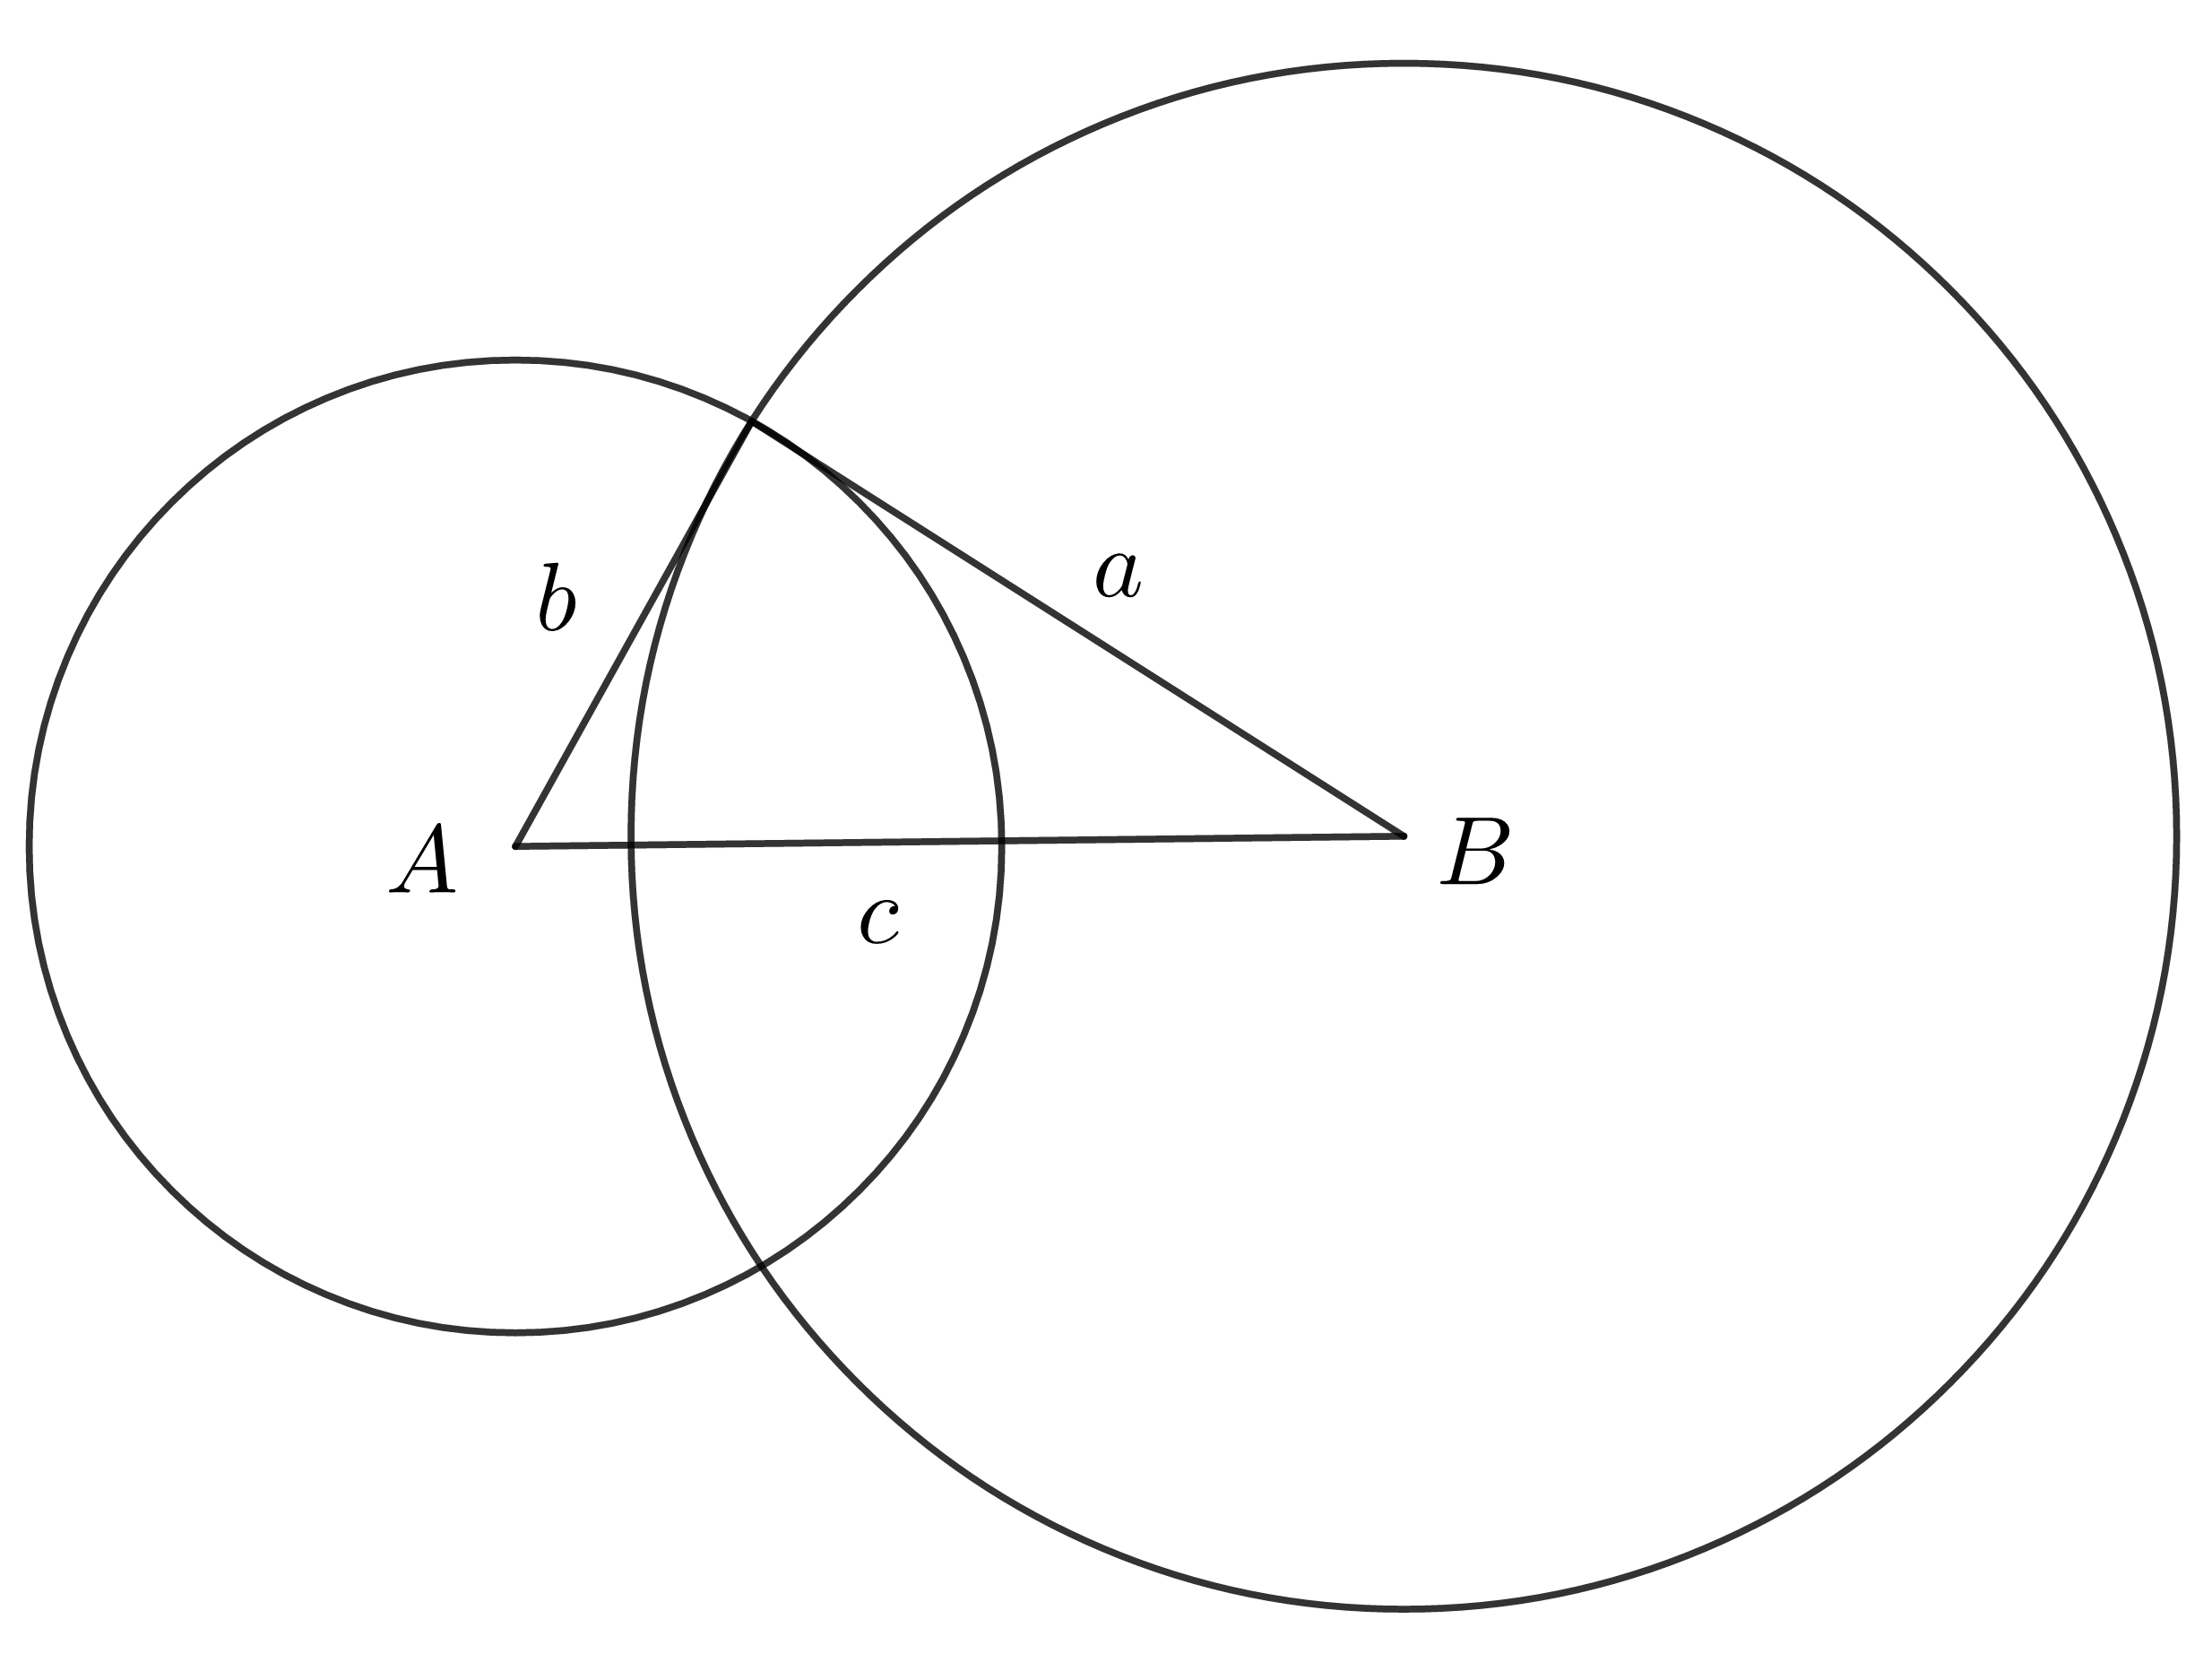
\includegraphics[scale=0.45]{Imagenes/demo3.png} 
\end{center}
\begin{tabular}{p{15.9cm} p{1cm}}
\\Construimos un triángulo con lados iguales a $a, b$ y $c$. 
\\Podemos suponer que $a \leq b \leq c$ y consideramos un segmento $AB$ de longitud $c$.
\\Trazamos ahora dos circunferencias una con centro en $A$ y radio $b$ y otra con centro en $B$ y radio $a$.
\\Como $c<a+b$, las dos circunferencias se intersectan (en caso contrario se tendría que $a+b \leq c)$. Uno de los puntos de intersección sirve como el tercer vértice $C$, del triángulo buscando $ABC$.
\end{tabular}
\begin{center}
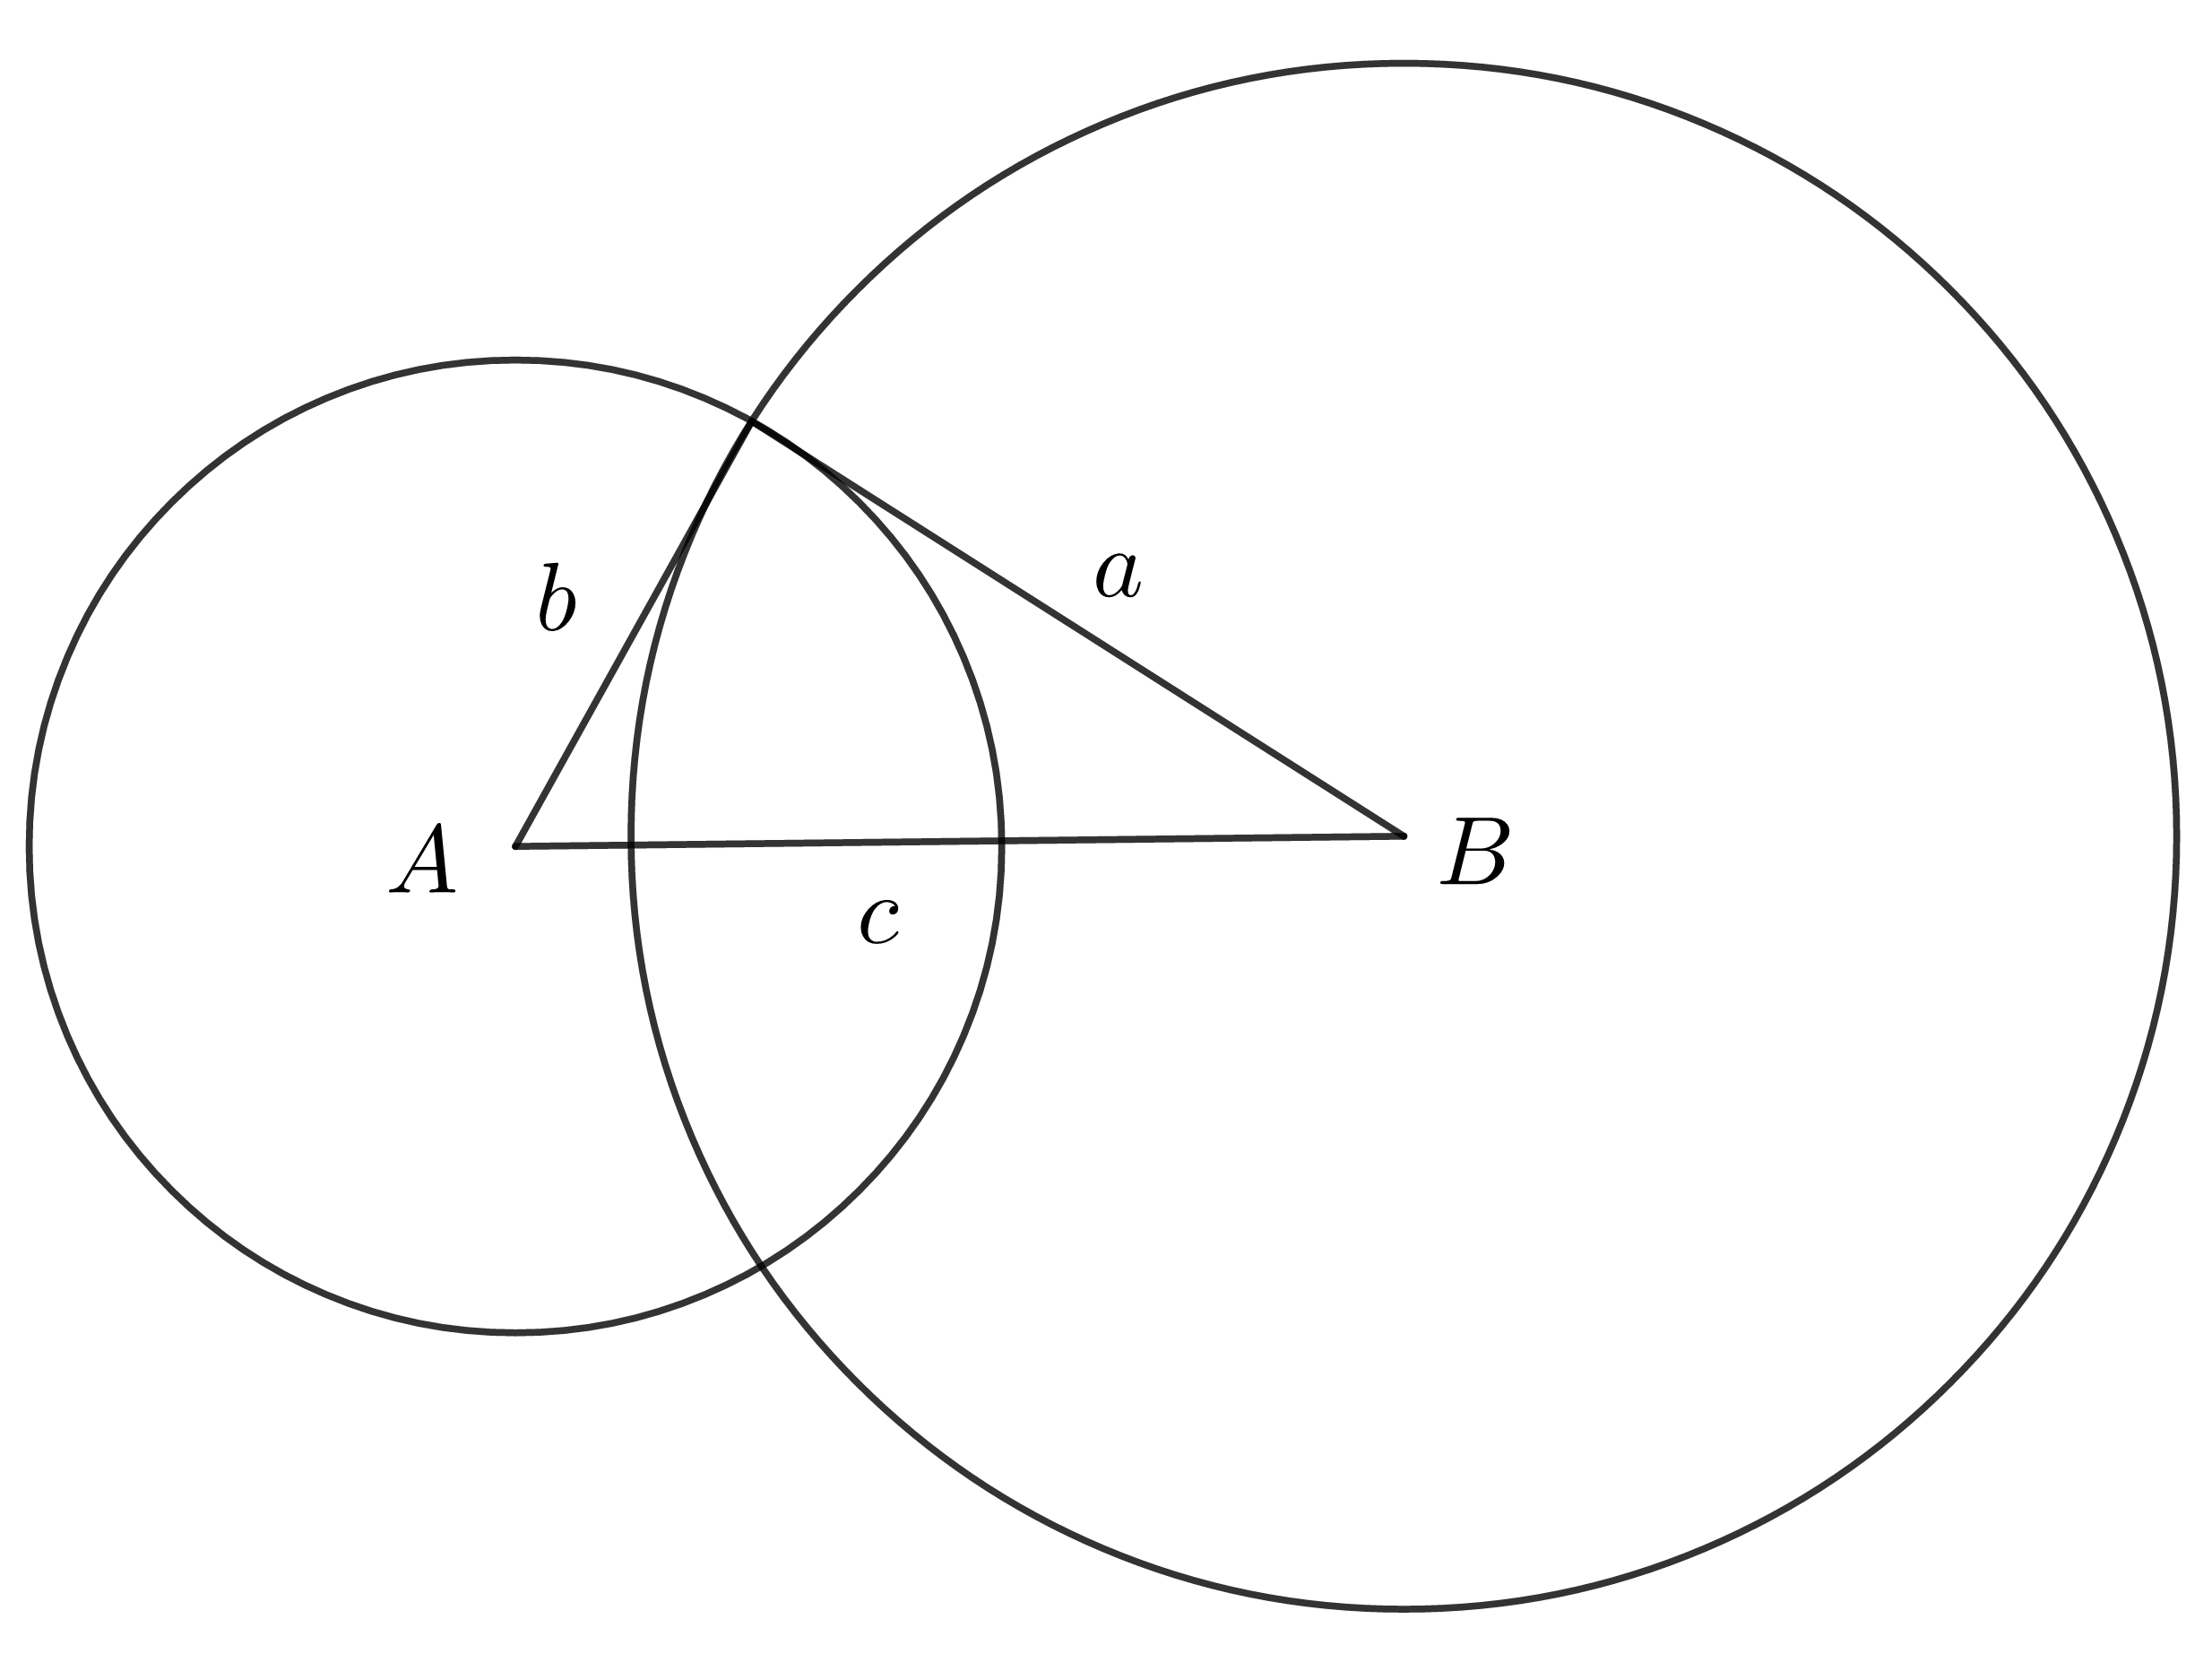
\includegraphics[scale=0.45]{Imagenes/demo3.png} 
\end{center}
\begin{tabular}{p{15.9cm} p{1cm}}
\\Construimos un triángulo con lados iguales a $a, b$ y $c$. 
\\Podemos suponer que $a \leq b \leq c$ y consideramos un segmento $AB$ de longitud $c$.
\\Trazamos ahora dos circunferencias una con centro en $A$ y radio $b$ y otra con centro en $B$ y radio $a$.
\\Como $c<a+b$, las dos circunferencias se intersectan (en caso contrario se tendría que $a+b \leq c)$. Uno de los puntos de intersección sirve como el tercer vértice $C$, del triángulo buscando $ABC$.
\end{tabular}
\end{document} 
